% ============================================================
% ANEXO C · FIGURAS COMPLEMENTARIAS
% Figuras metodológicas y experimentales que complementan el cuerpo del reporte.
% Decisiones y hallazgos que las respaldan: H-016, H-018, H-019, H-020,
% H-036, H-041, H-044, H-049, D-014, D-022, D-031.
% ============================================================

\section{Figuras complementarias}\label{anx:figuras}

En esta sección se compilan aquellas figuras generadas durante las fases de caracterización,
evaluación de complejidad y análisis exploratorio del pipeline que, por razones de espacio y
fluidez narrativa, no fueron incluidas en los capítulos metodológicos ni de resultados principales.
Las figuras relativas a la distribución exploratoria de variables clínicas e imágenes DICOM
del conjunto de datos se presentan en el anexo correspondiente.

% ------------------------------------------------------------
\subsection{Preprocesamiento e imágenes de entrada}

\begin{figure}[H]
\centering
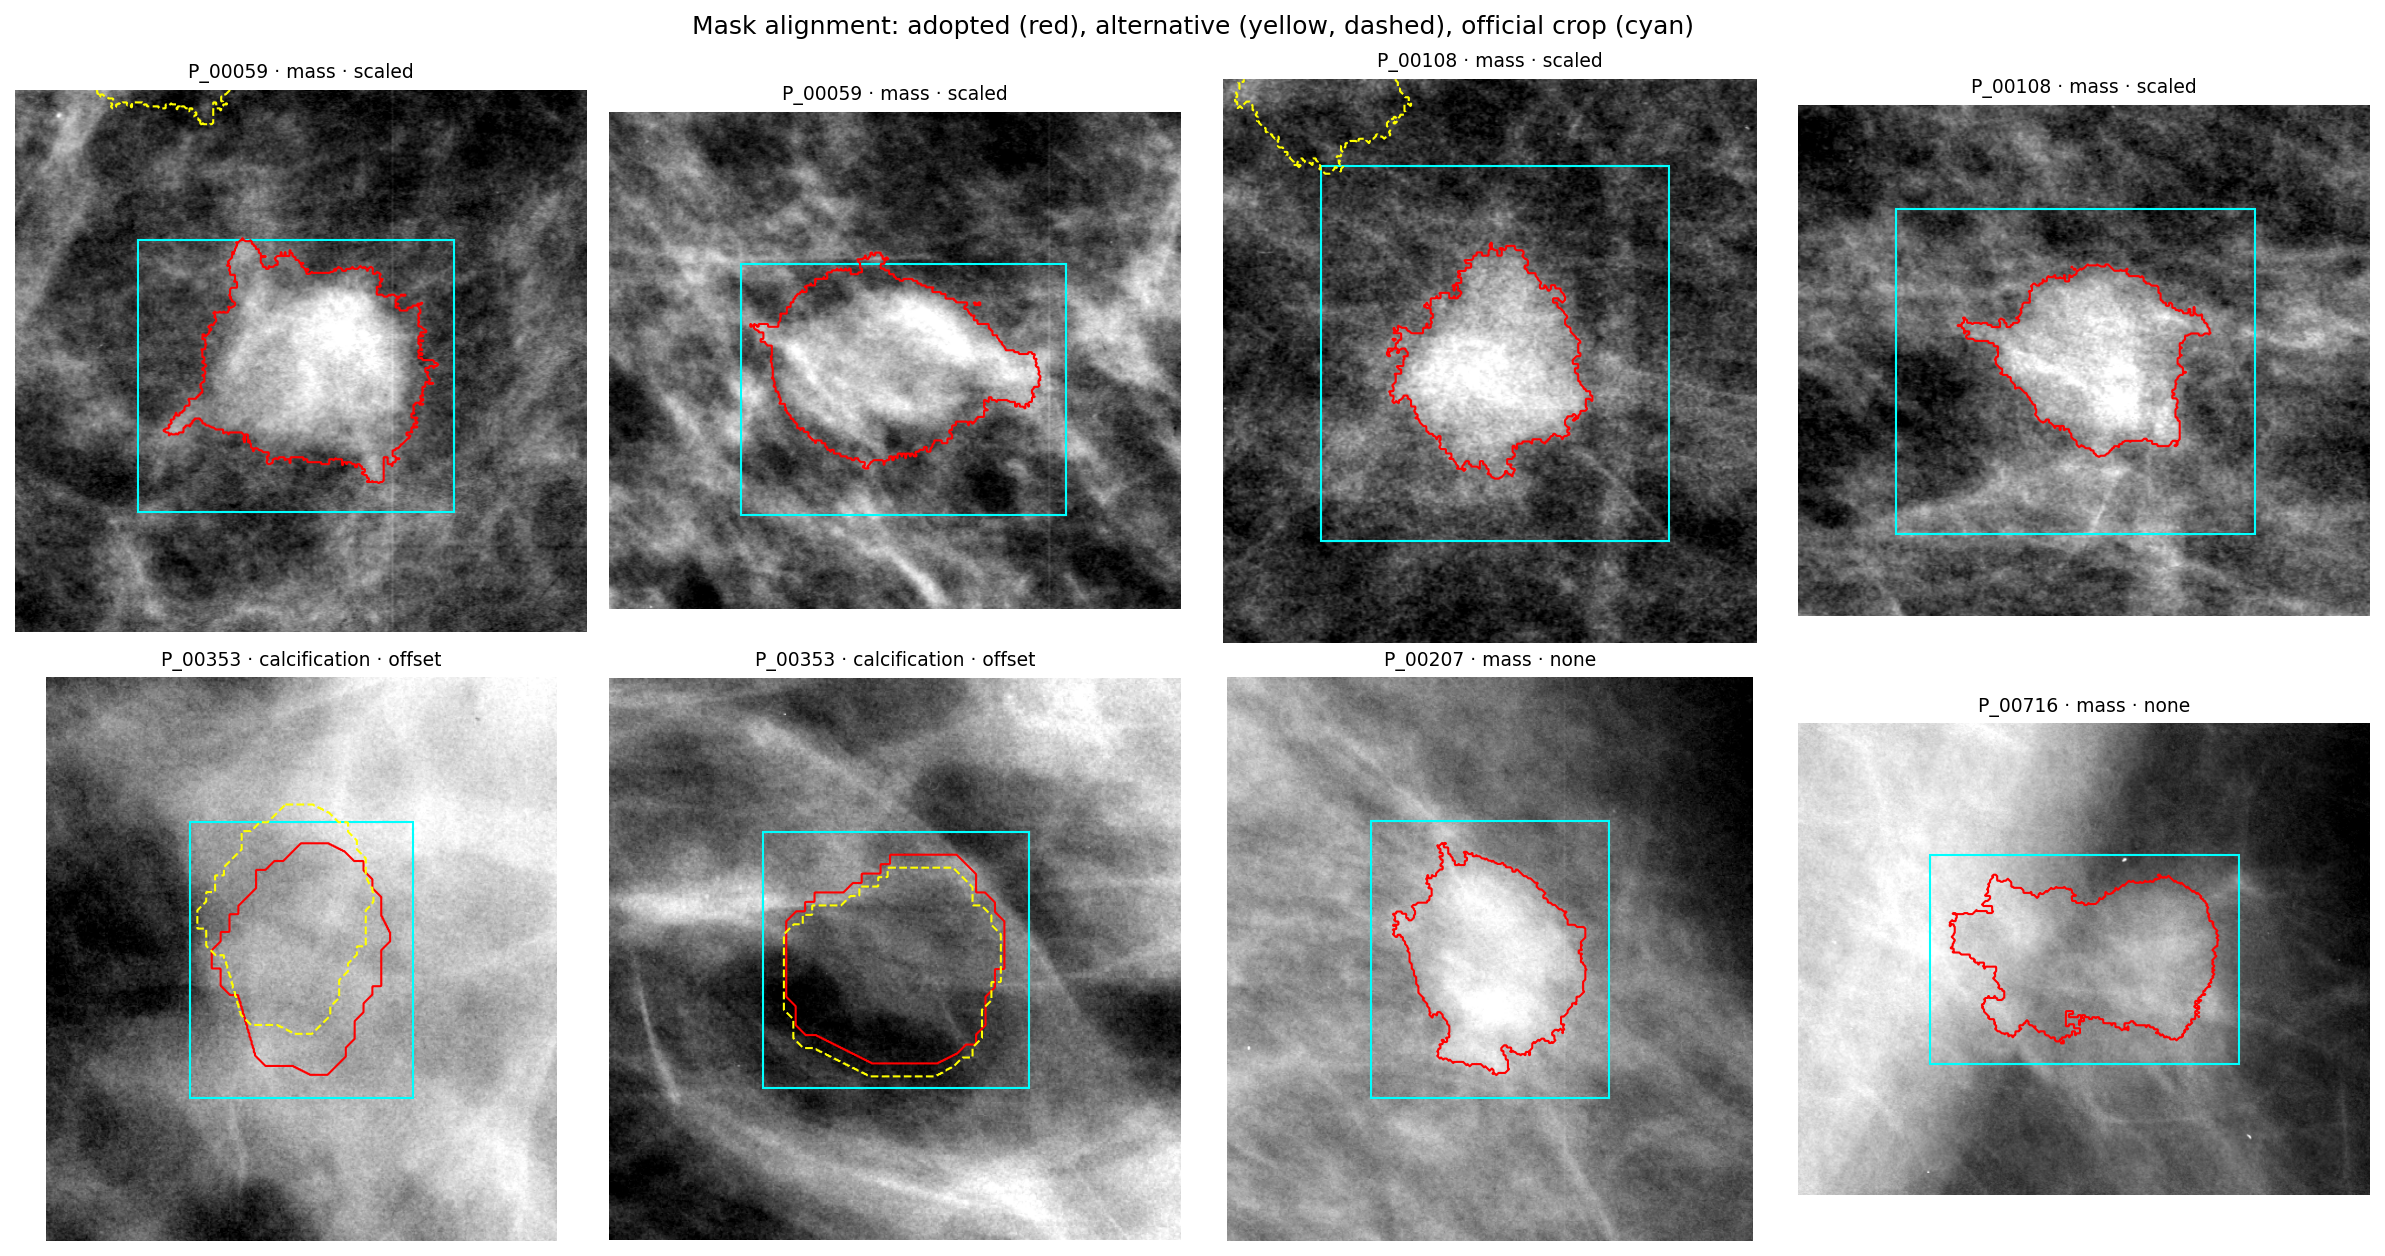
\includegraphics[width=\textwidth]{Figures/M2_mask_alignment.png}
% fuente: H-020
\caption{Diagnóstico de desajuste dimensional y verificación de alineación espacial de máscaras en el Módulo 2. Se ilustran los dos casos identificados: discordancia por factor de escala ($0.870$) y desajuste por traslación de origen, contrastados con el recorte oficial.}
\label{fig:anx_m2_alignment}
\end{figure}

\begin{figure}[H]
\centering
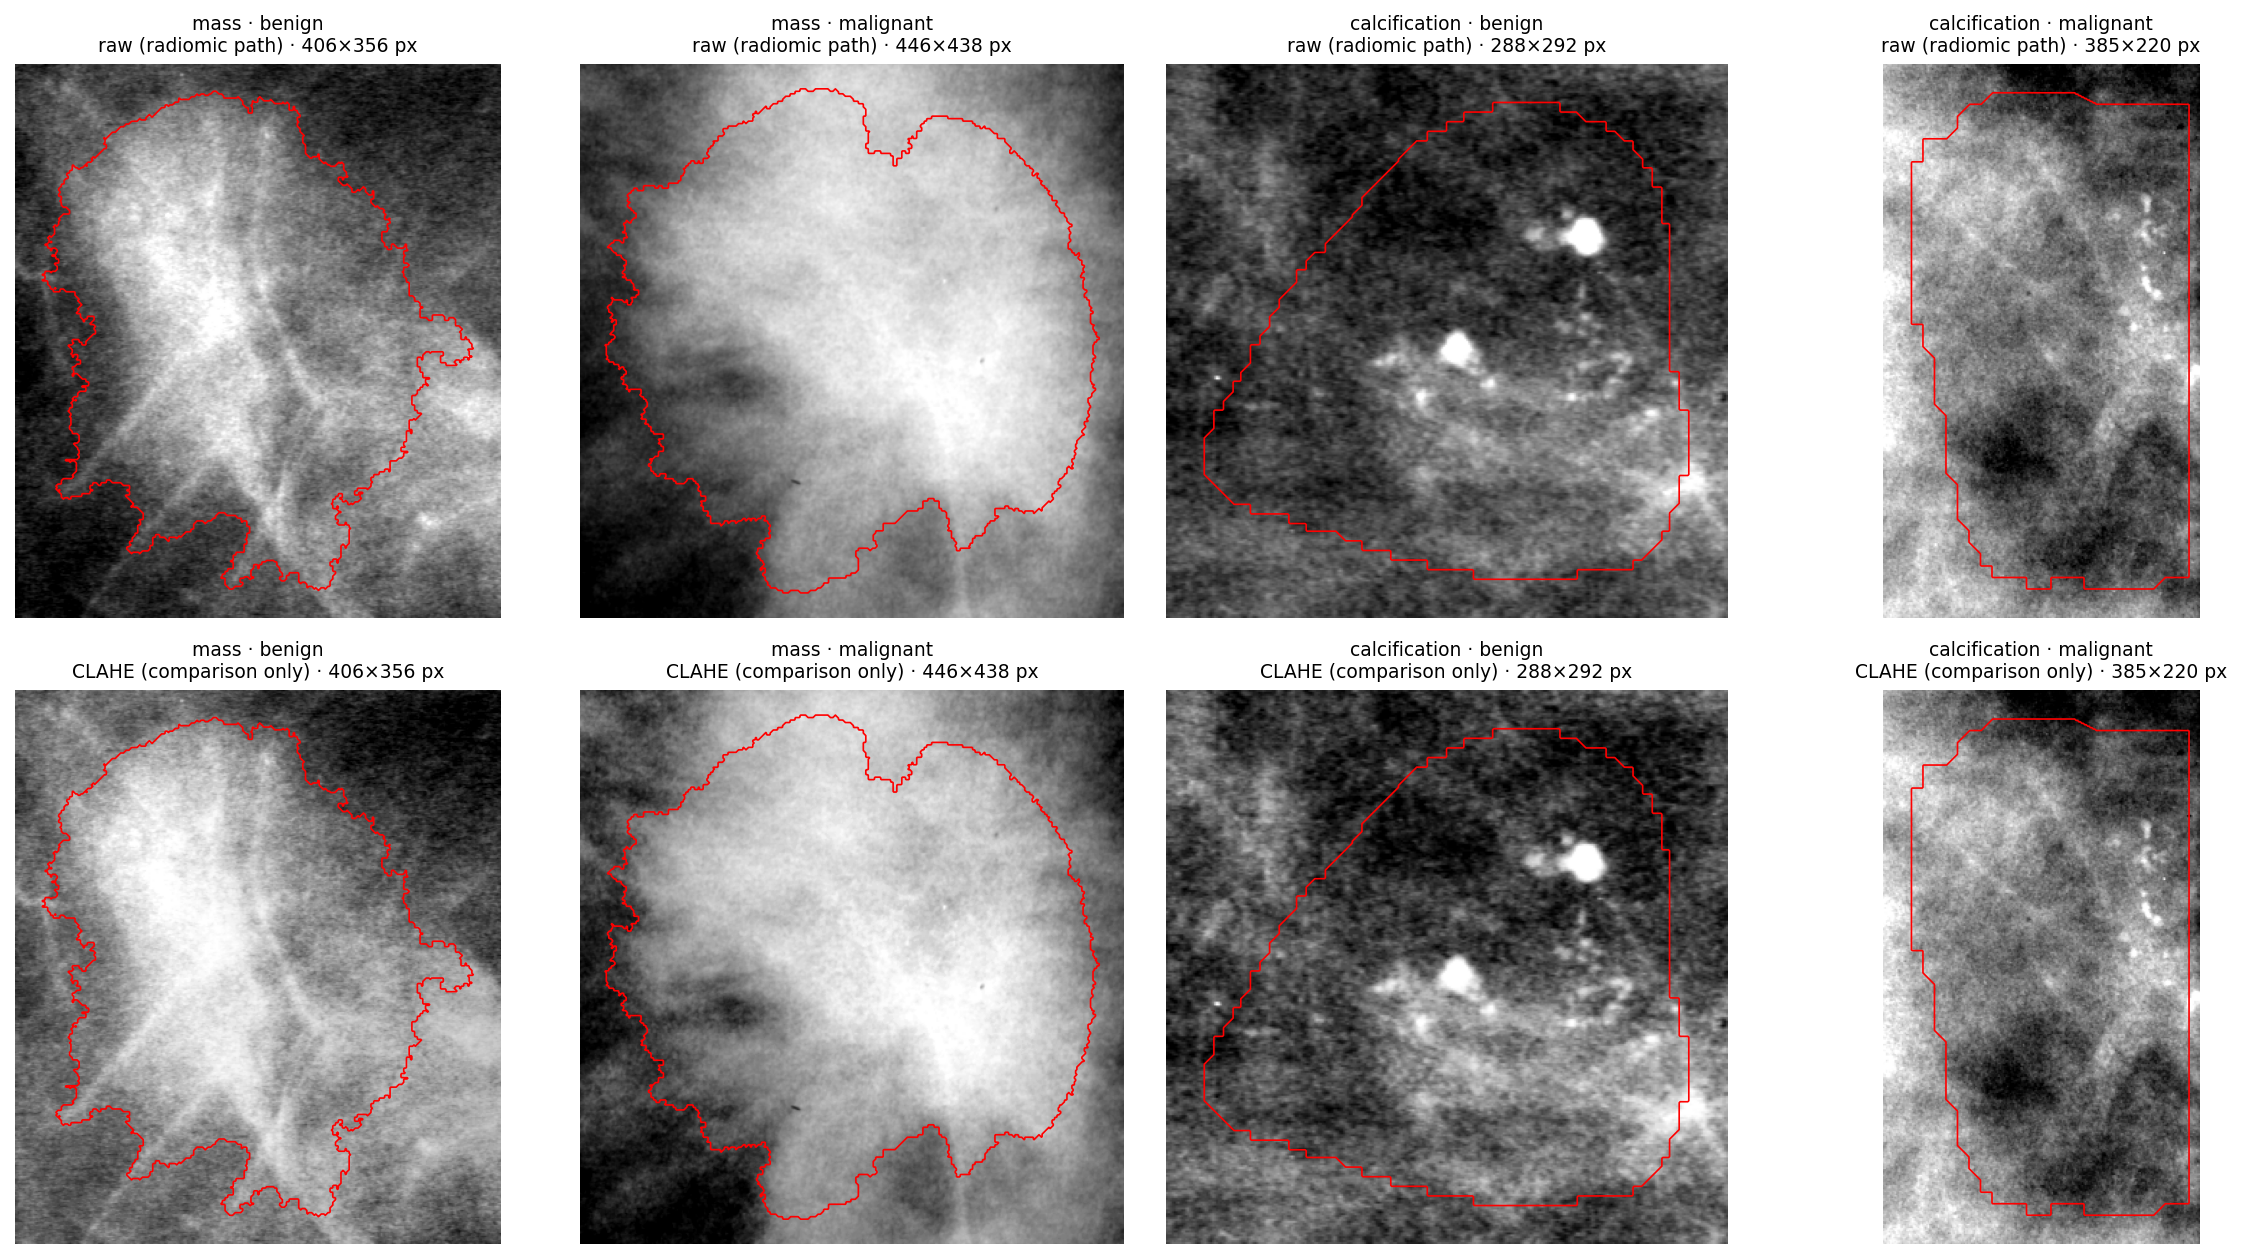
\includegraphics[width=\textwidth]{Figures/M2_preprocessing_examples.png}
% fuente: D-022
\caption{Ejemplos ilustrativos de las etapas de preprocesamiento sobre mamografías del CBIS-DDSM (Módulo 2). Se muestra la mamografía completa, la máscara binarizada depurada, la región de interés recortada con margen de seguridad y su correspondiente versión procesada mediante ecualización CLAHE.}
\label{fig:anx_m2_examples}
\end{figure}

% ------------------------------------------------------------
\subsection{Circuitos cuánticos y mapas de características}

\begin{figure}[H]
\centering
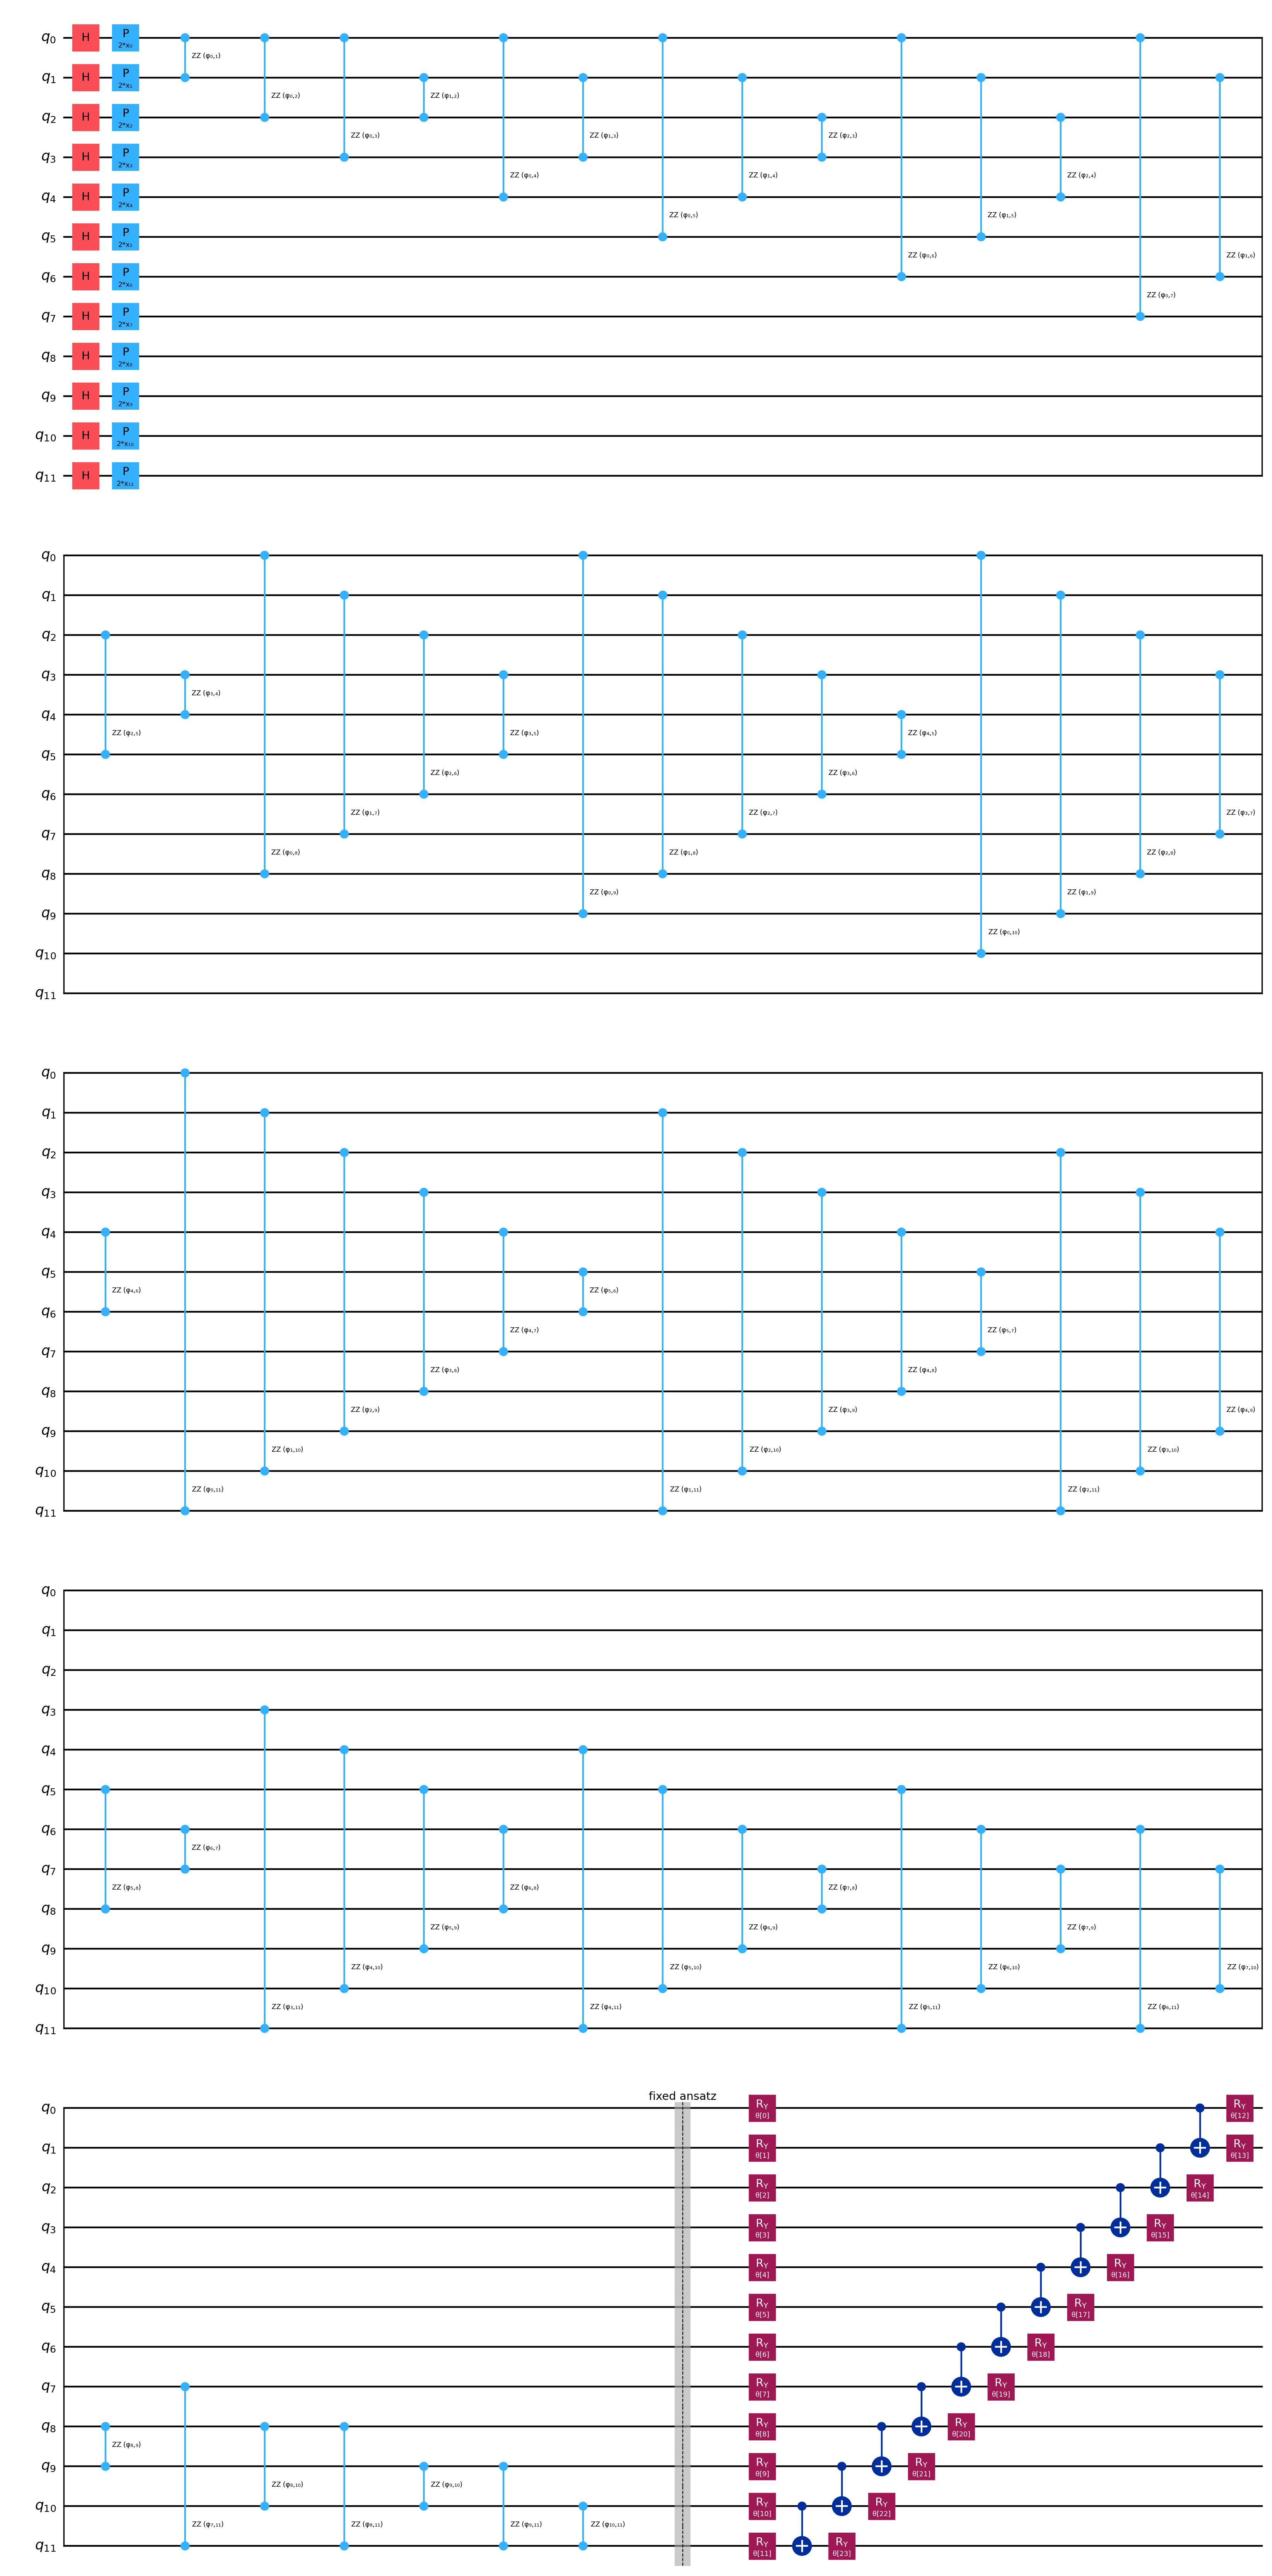
\includegraphics[width=0.6\textwidth]{Figures/M5_circuit_12q.png}
% fuente: D-031
\caption{Diagrama esquemático completo del circuito cuántico variacional implementado para $k = 12$ qubits (Módulo 5). Incluye la codificación angular de características, el entrelazamiento completo de dos qubits y la capa variacional con \textit{ansatz} \texttt{RealAmplitudes} de una repetición parametrizada con vector $\theta$ fijo.}
\label{fig:anx_m5_circuit_12q}
\end{figure}

\begin{figure}[H]
\centering
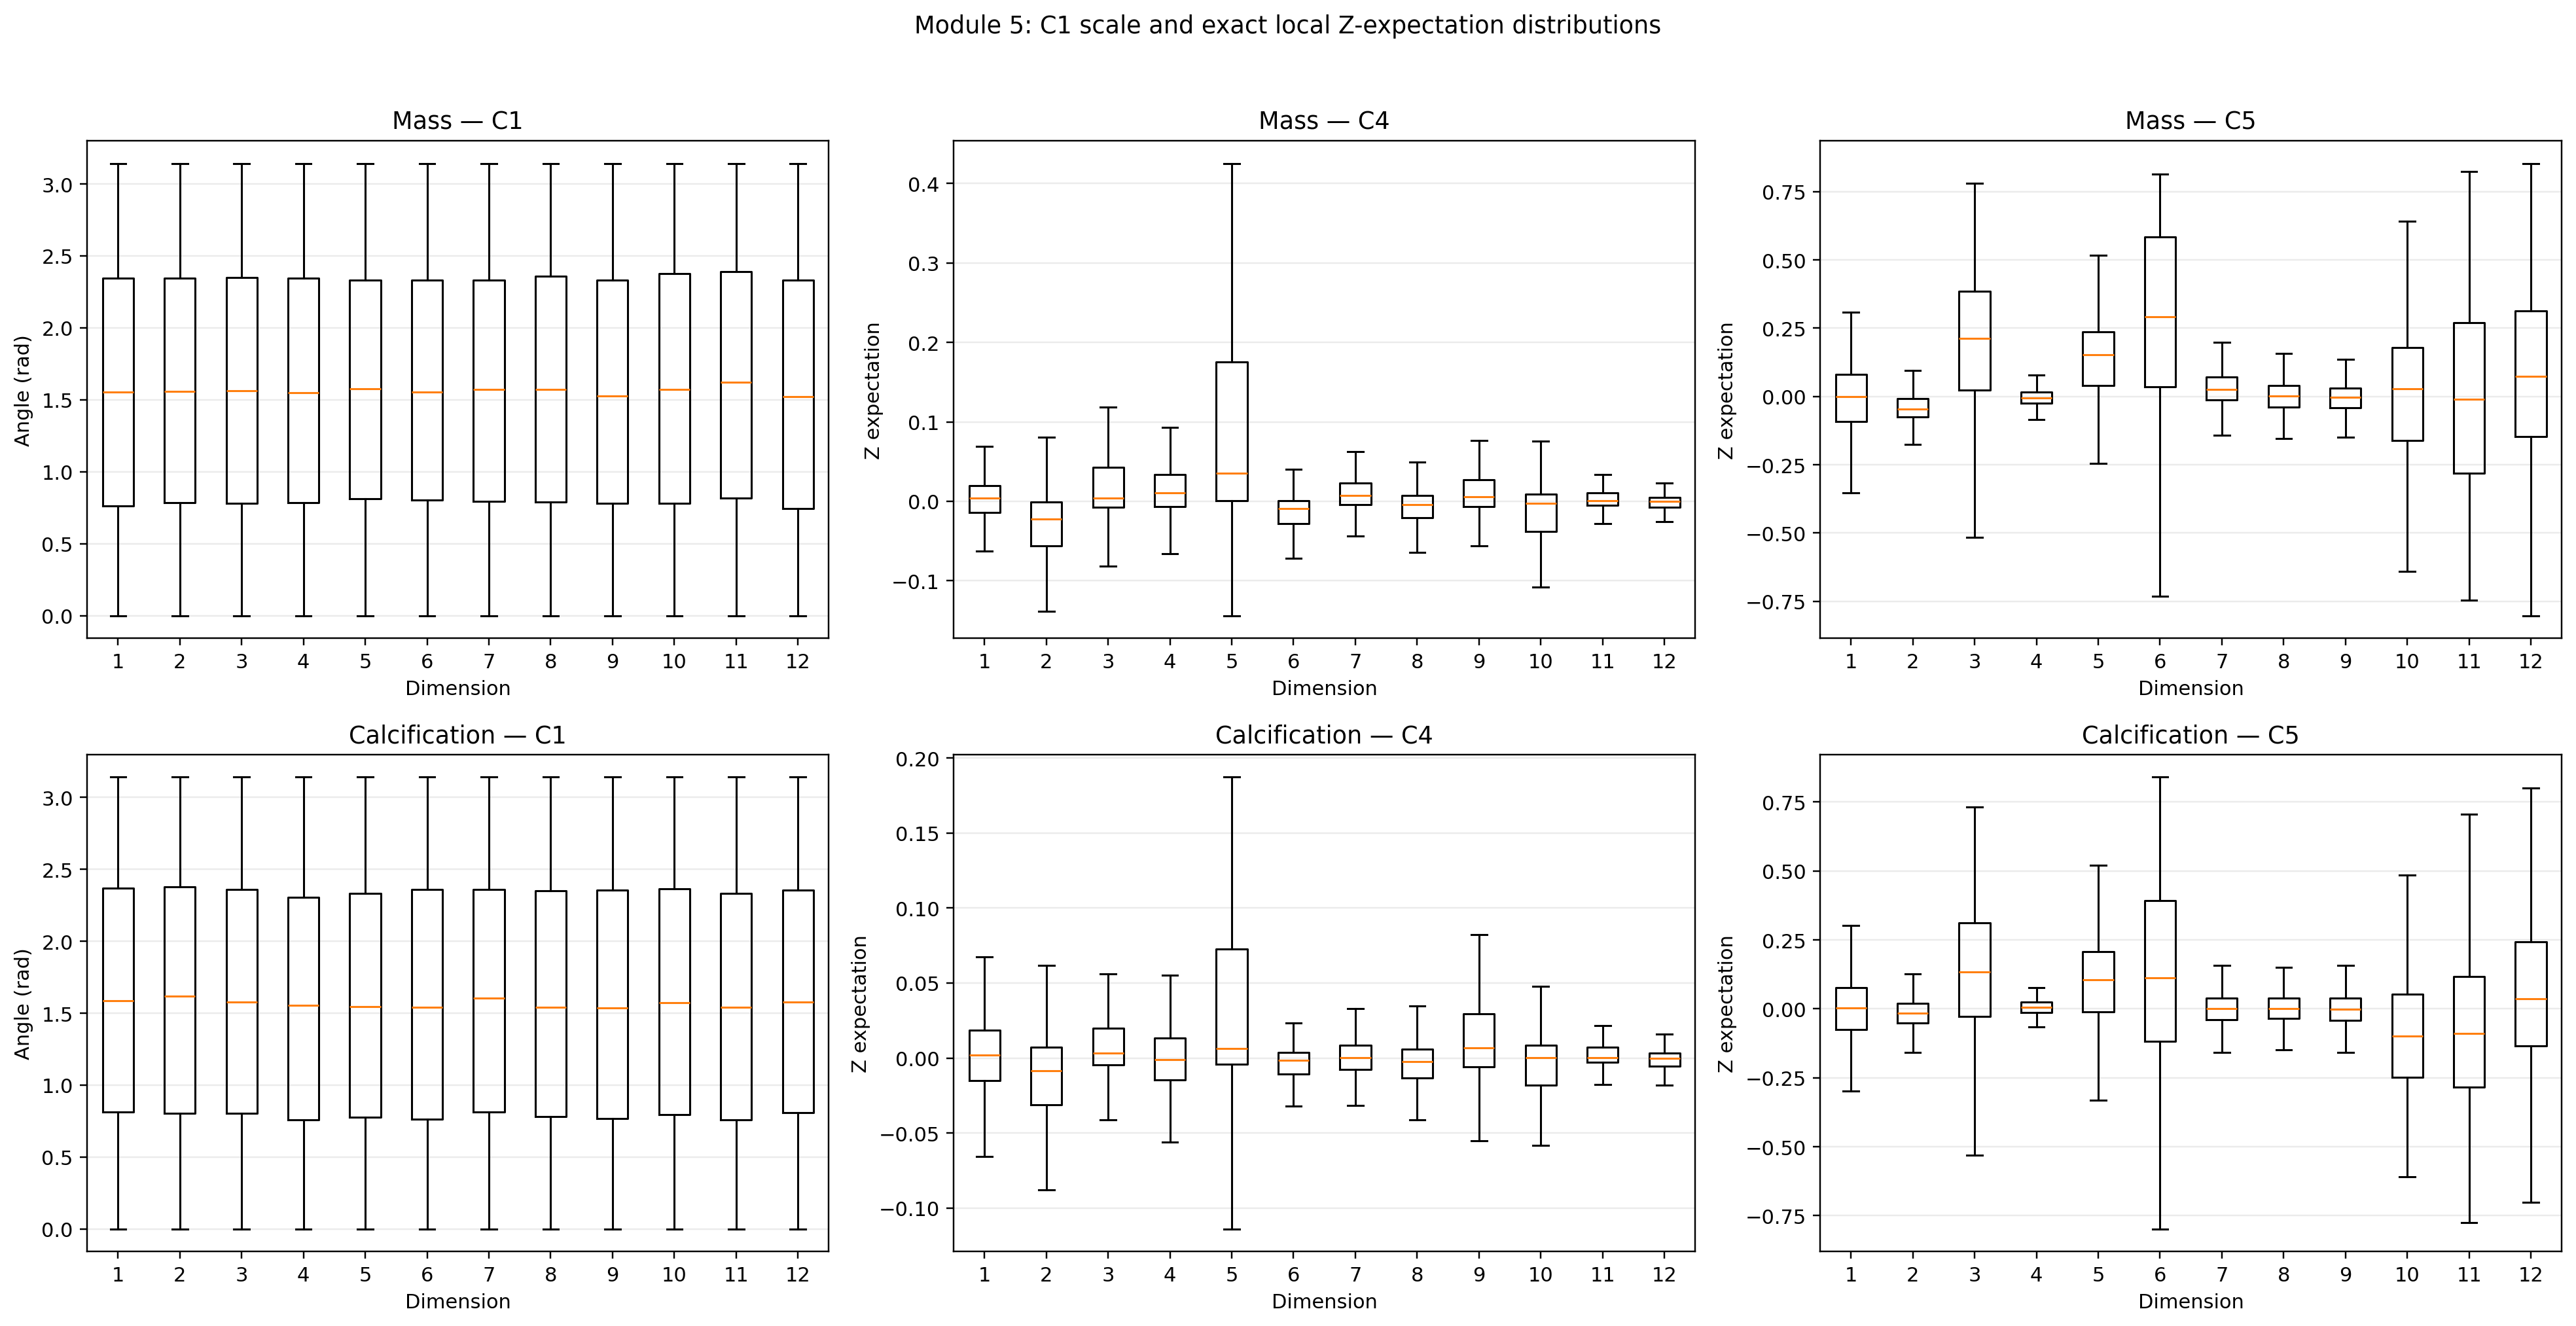
\includegraphics[width=\textwidth]{Figures/M5_embeddings.png}
% fuente: D-014
\caption{Distribución empírica de los valores esperados de Pauli locales $\langle Z_i \rangle$ generados por los mapas cuánticos C4 y C5 para cada dimensión del embedding en masas y calcificaciones (Módulo 5).}
\label{fig:anx_m5_embeddings}
\end{figure}

% ------------------------------------------------------------
\subsection{Complejidad, costes y muestreo de estados cuánticos}

\begin{figure}[H]
\centering
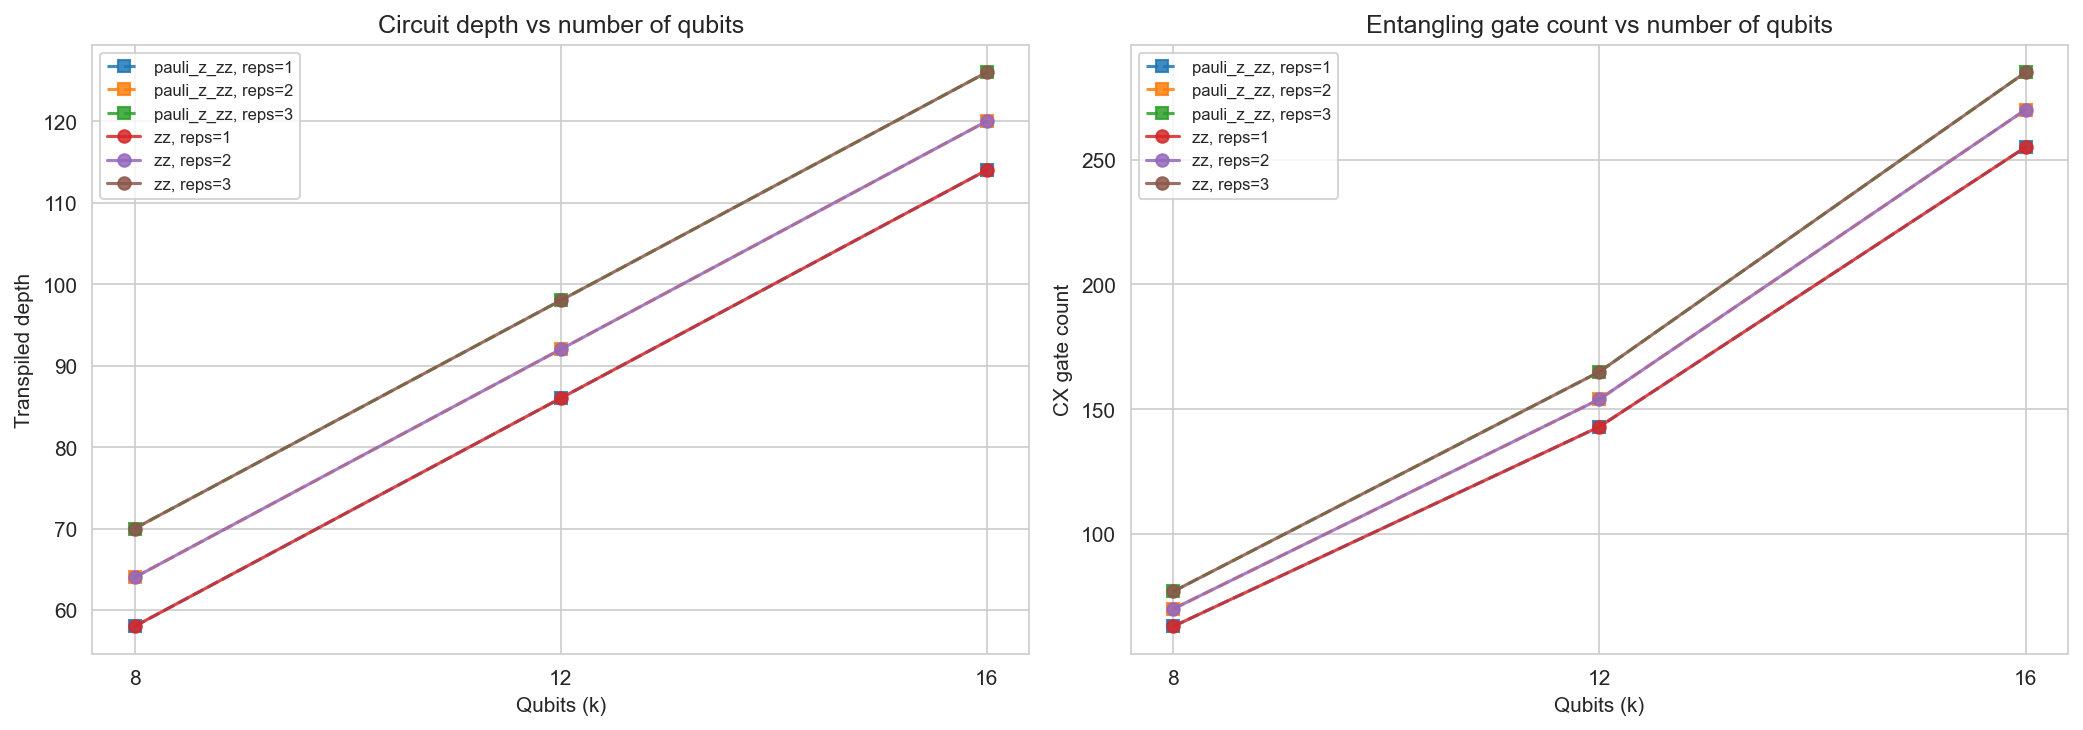
\includegraphics[width=\textwidth]{Figures/E1_circuit_complexity.png}
% fuente: D-013
\caption{Complejidad estructural de los circuitos cuánticos evaluados en función del número de qubits $k$. Se reporta la profundidad total del circuito y el número de compuertas de dos cúbits requeridas para distintas configuraciones.}
\label{fig:anx_e1_complexity}
\end{figure}

\begin{figure}[H]
\centering
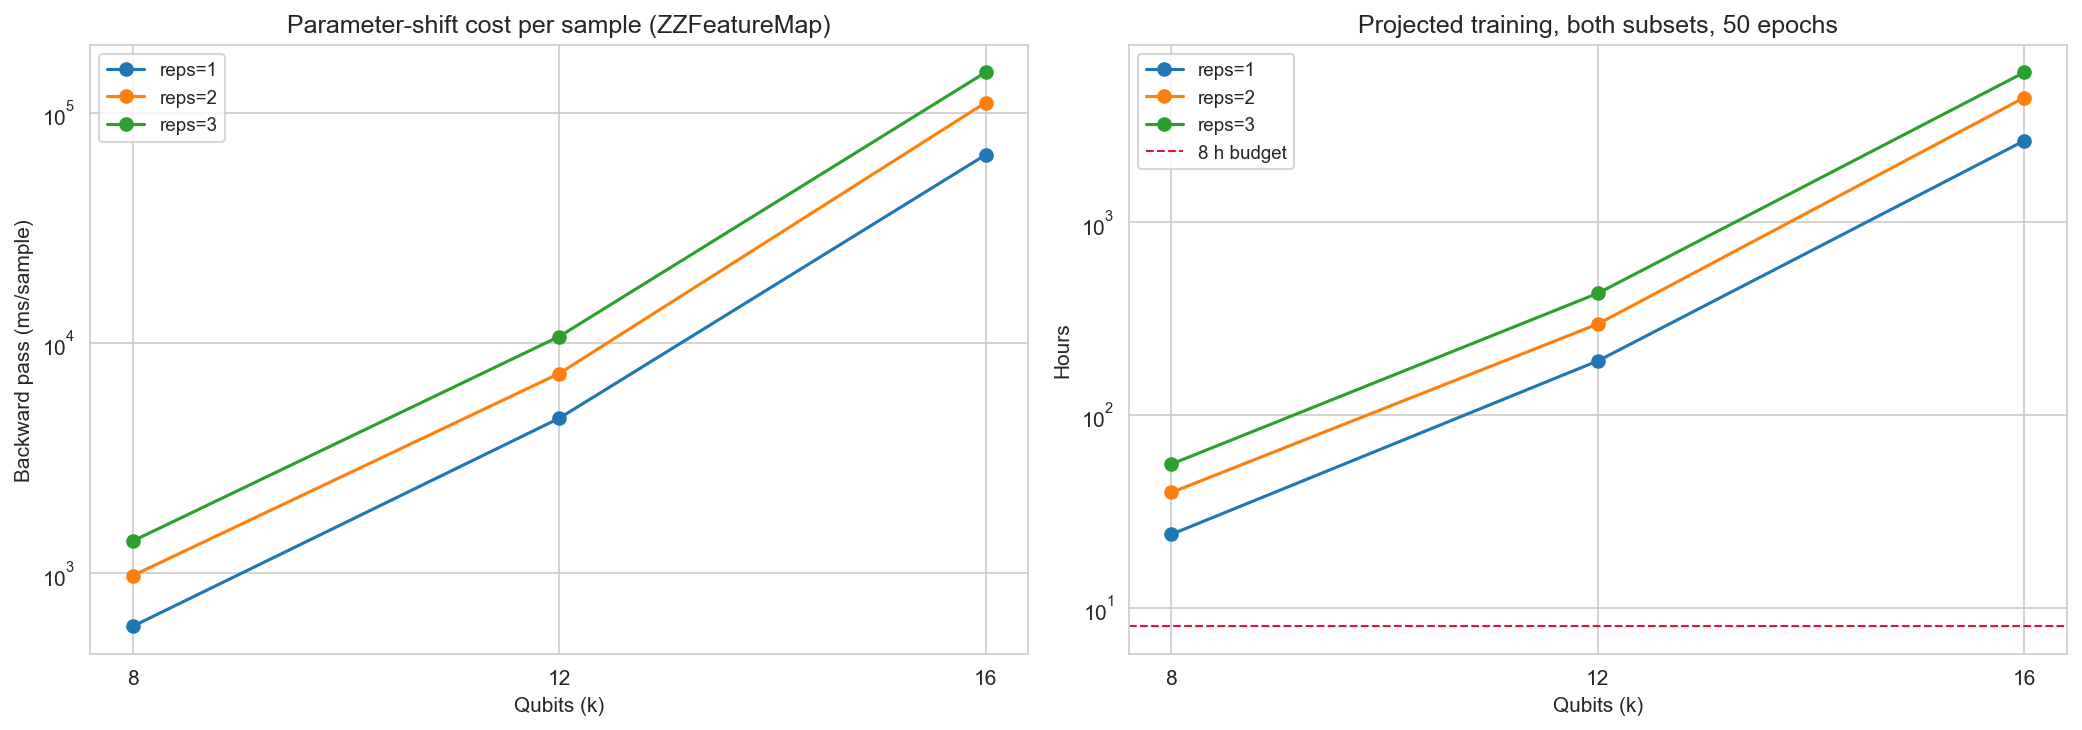
\includegraphics[width=\textwidth]{Figures/E2_training_cost.png}
% fuente: D-013
\caption{Coste computacional del entrenamiento variacional medido en segundos por época y muestra en simuladores cuánticos para diversas topologías de circuito y números de qubits.}
\label{fig:anx_e2_training_cost}
\end{figure}

\begin{figure}[H]
\centering
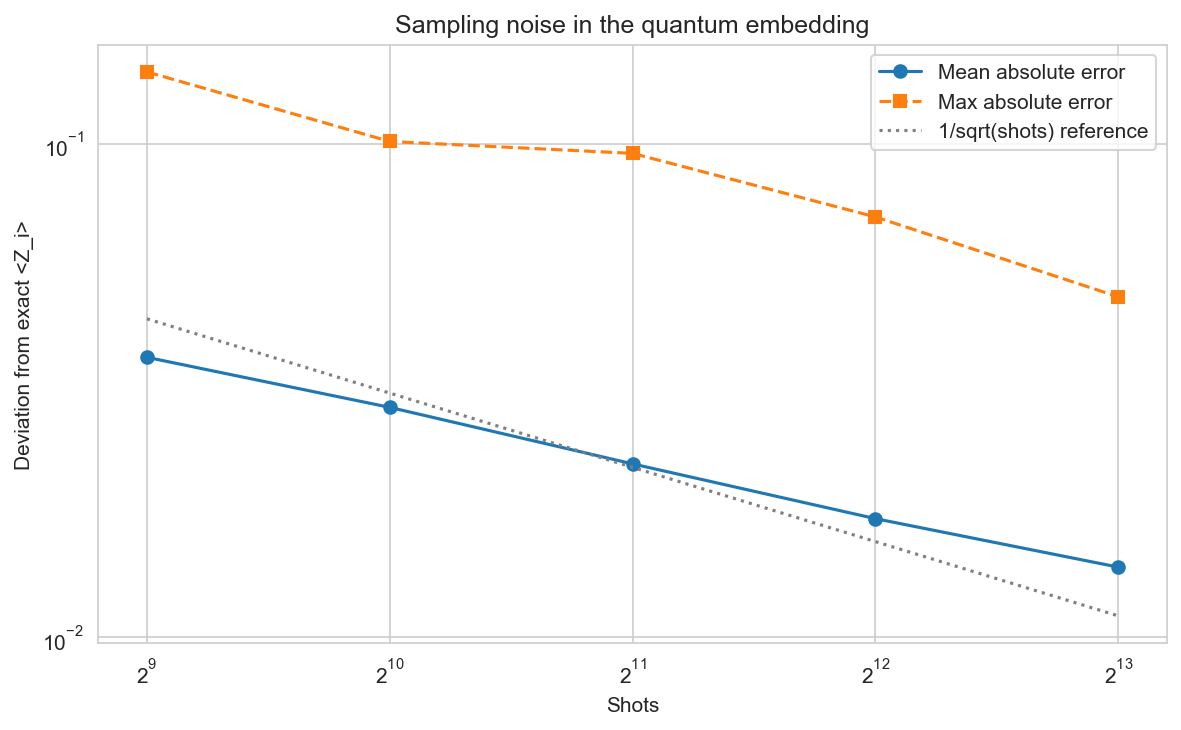
\includegraphics[width=\textwidth]{Figures/E3_shots_sensitivity.png}
% fuente: H-016, H-019
\caption{Sensibilidad del error de estimación al número de disparos finitos (\textit{shots}). El aparente estancamiento en precisión observado en la versión preliminar de este análisis respondió a ruido numérico en la referencia de evaluación, según se documentó y subsanó posteriormente en el cuaderno B3 con cálculos exactos.}
\label{fig:anx_e3_shots}
\end{figure}

\begin{figure}[H]
\centering
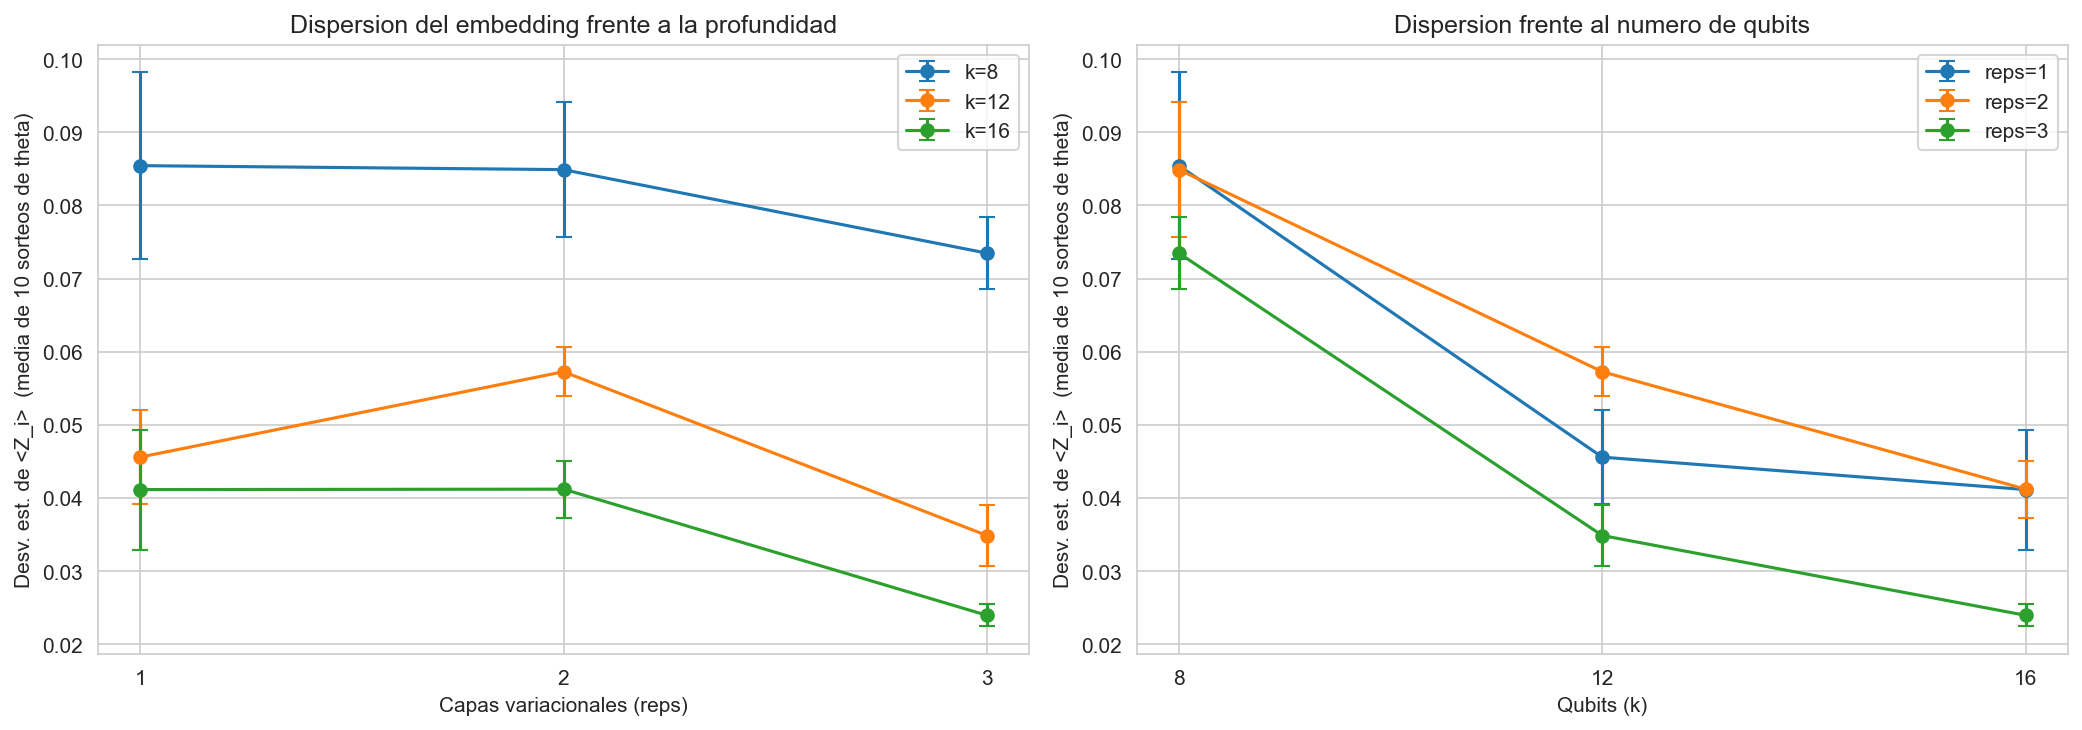
\includegraphics[width=\textwidth]{Figures/E4_embedding_concentration.png}
% fuente: H-018
\caption{Efecto de concentración de medida en el espacio de Hilbert al incrementar el número de qubits $k$. La dispersión entre estados para diferentes lesiones decae exponencialmente conforme aumenta la dimensionalidad cuántica.}
\label{fig:anx_e4_concentration}
\end{figure}

% ------------------------------------------------------------
\subsection{Experimentos complementarios de kernels, dimensionalidad y QSVM}

\begin{figure}[H]
\centering
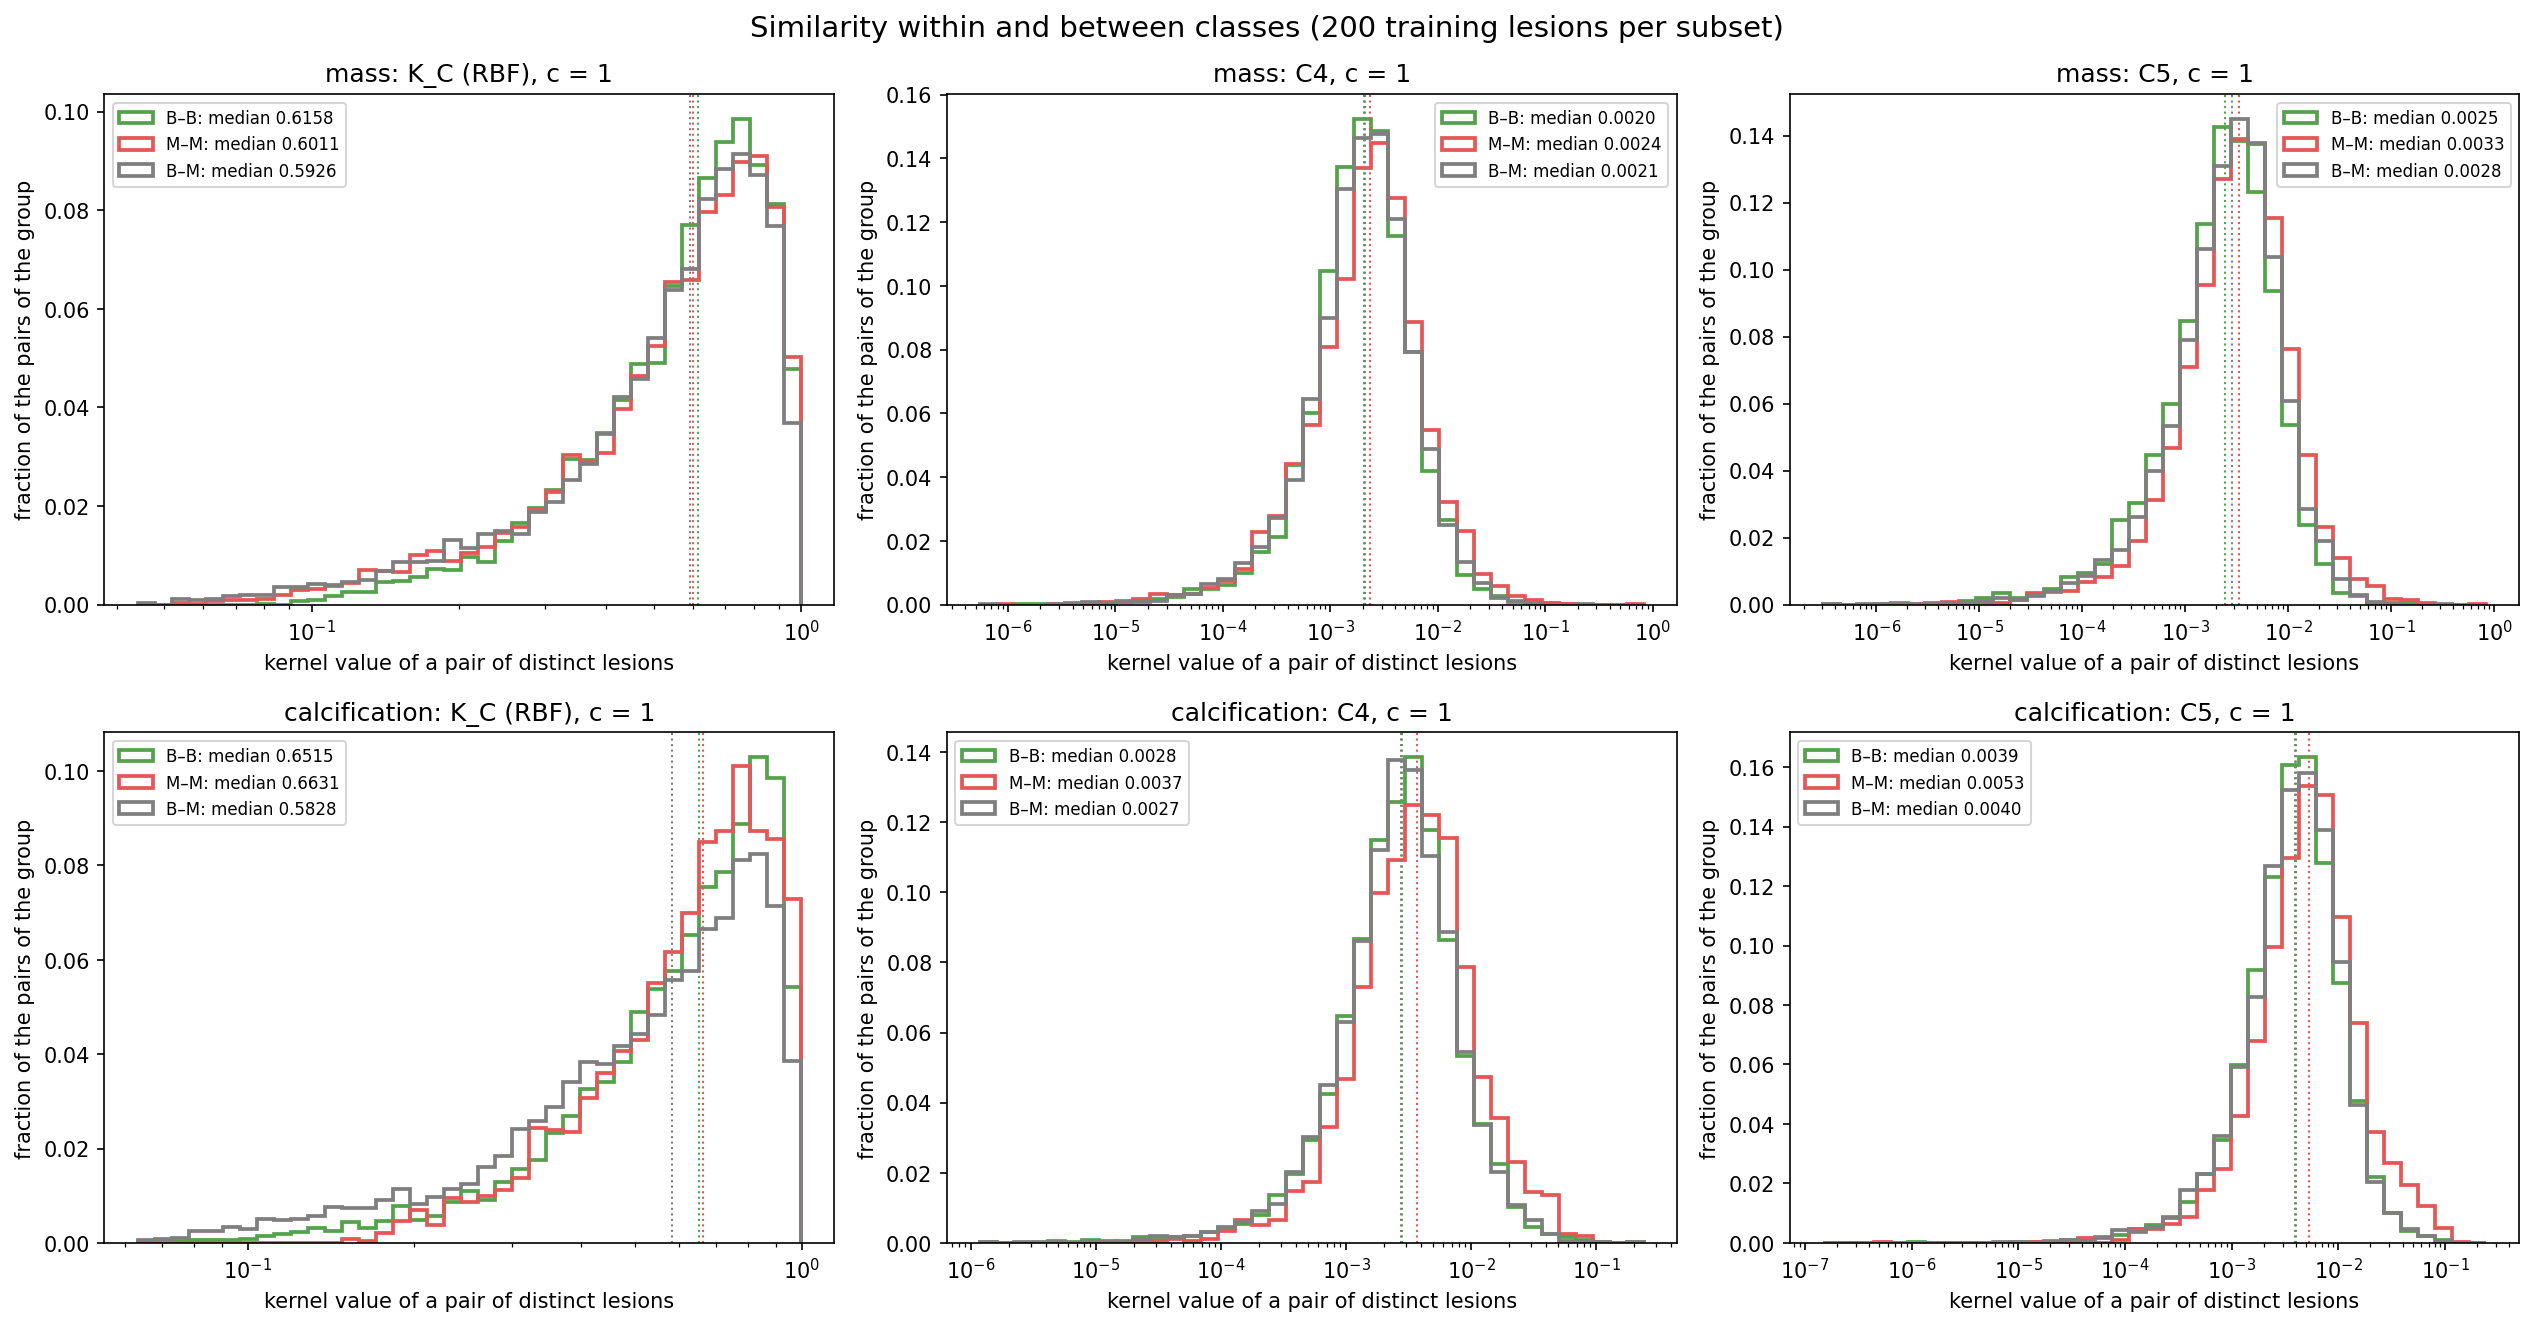
\includegraphics[width=\textwidth]{Figures/X2_kernel_pairs_by_class.png}
% fuente: H-036
\caption{Distribución de valores de similitud en matrices de kernel intraclase e interclase (Experimento X2). Se compara la discriminación obtenida por el kernel clásico RBF frente a los mapas cuánticos C4 y C5 bajo distintos factores de escala angular $c$.}
\label{fig:anx_x2_pairs}
\end{figure}

\begin{figure}[H]
\centering
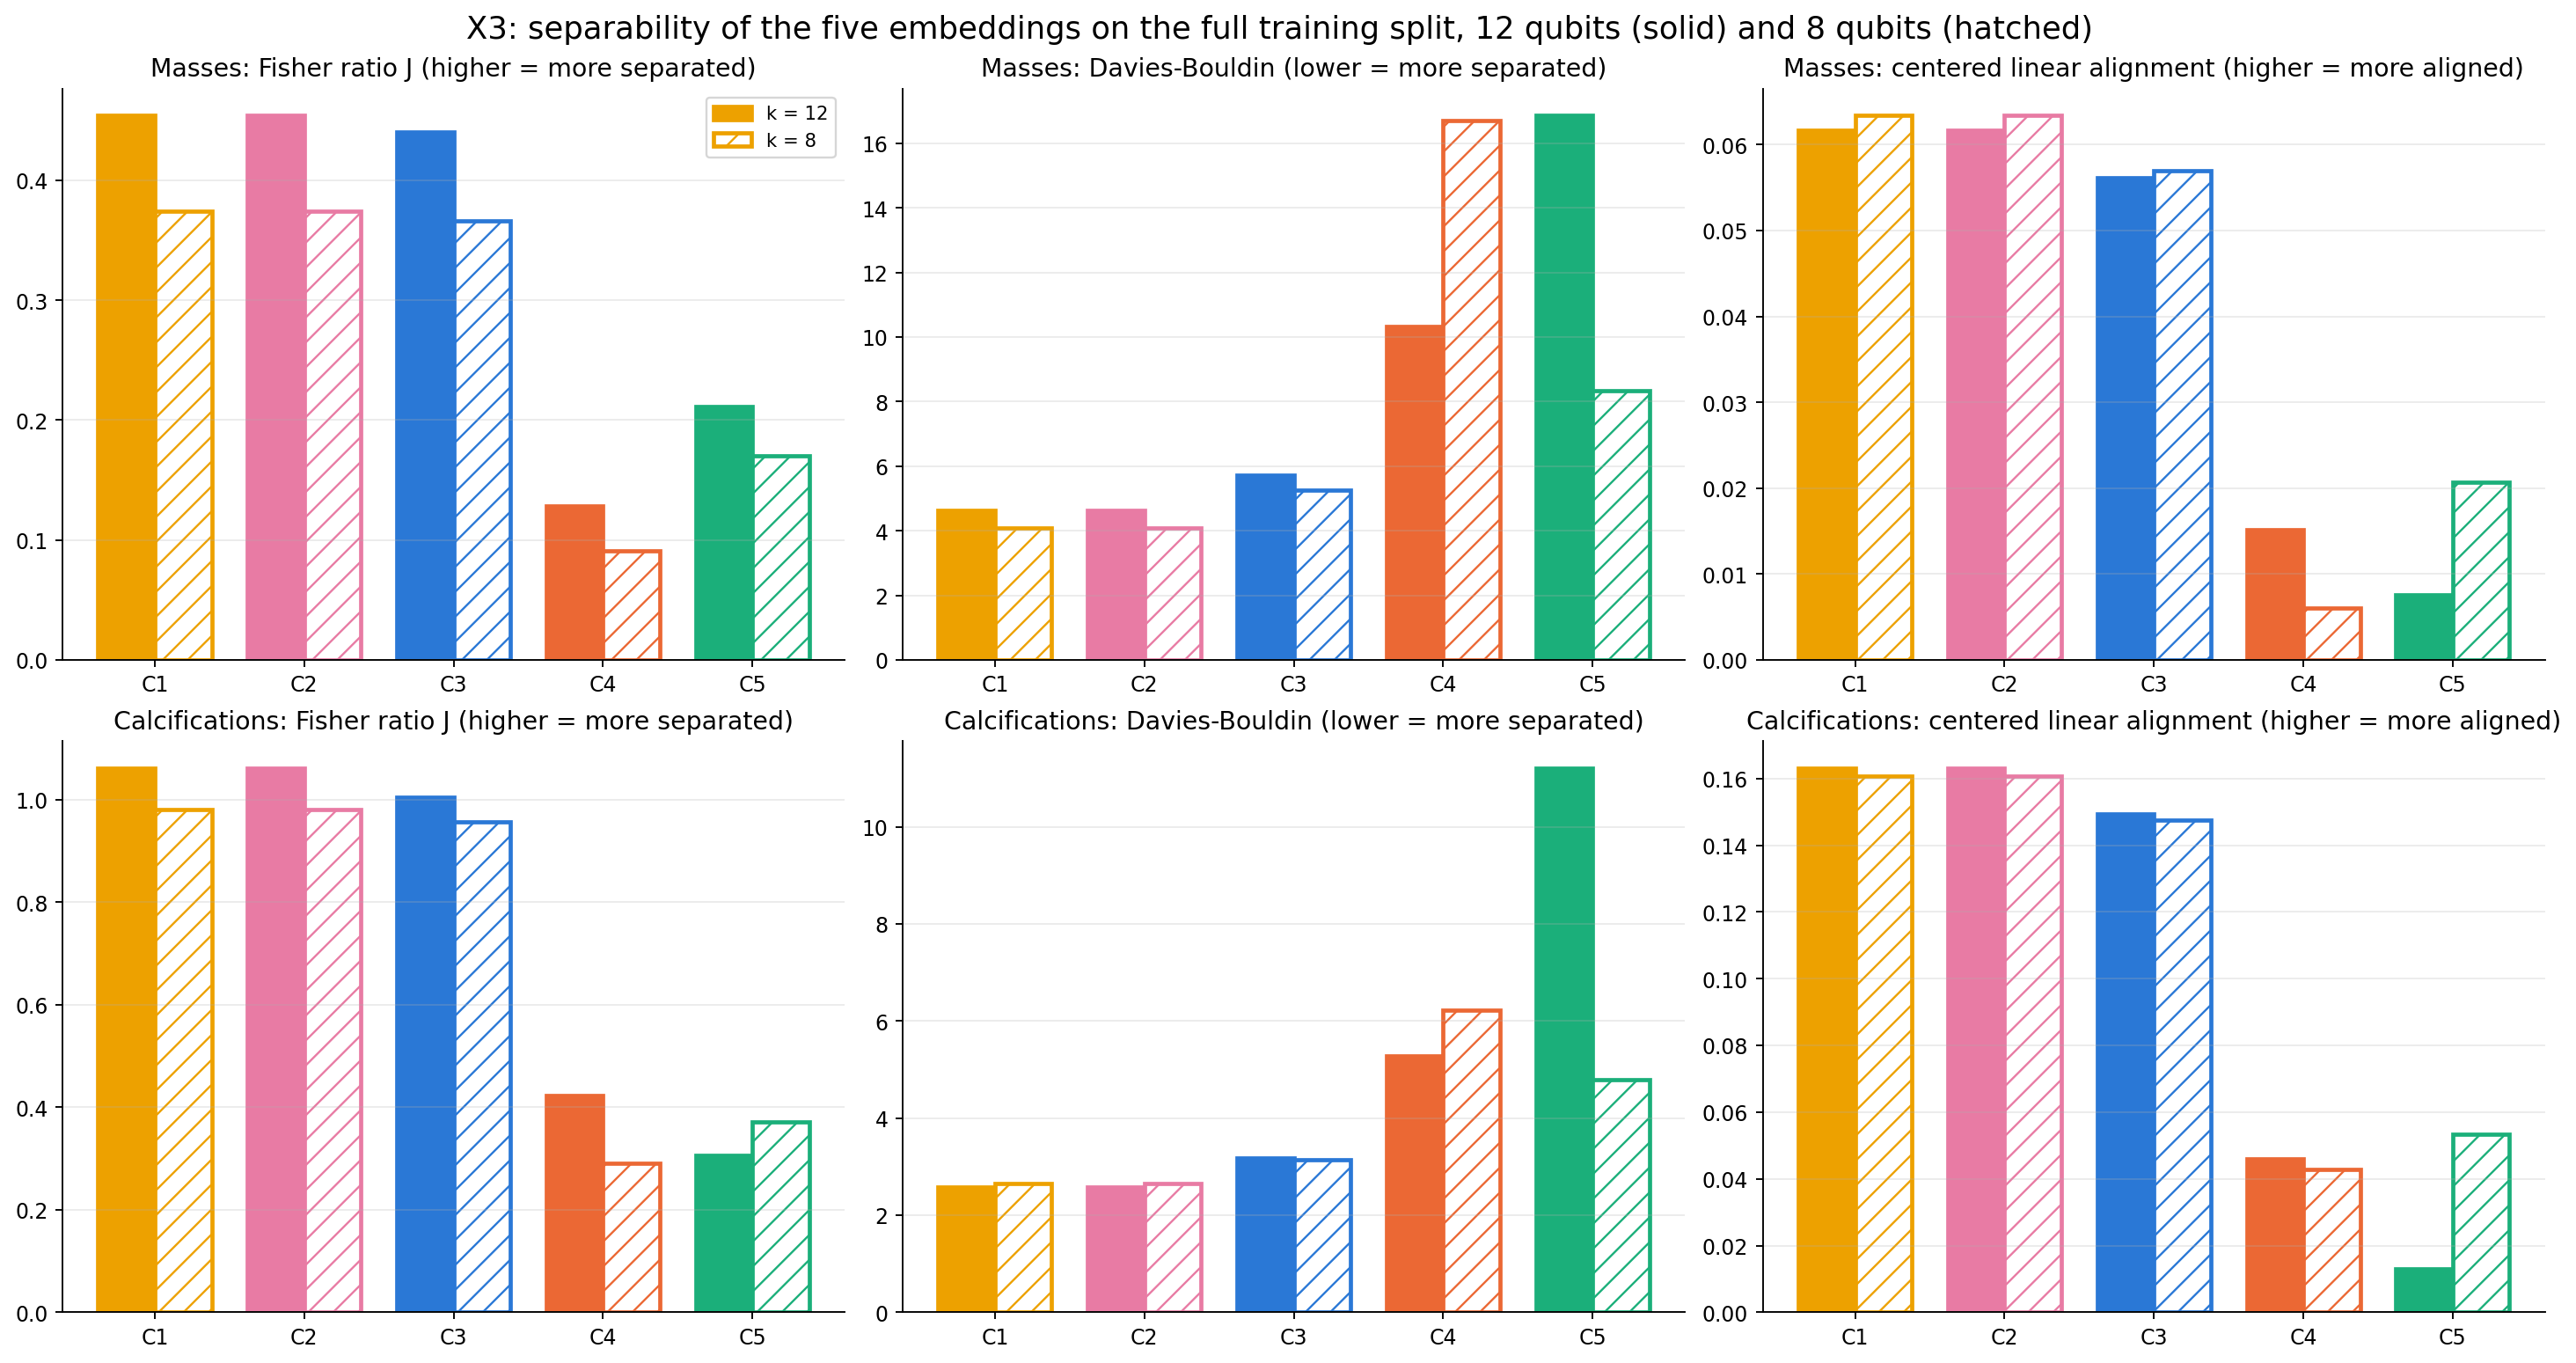
\includegraphics[width=\textwidth]{Figures/X3_embedding_metrics_k8_k12.png}
% fuente: H-041
\caption{Comparativa de métricas de separabilidad geométrica (Davies--Bouldin, Fisher $J$ y alineamiento KTA) entre la configuración reducida de $k = 8$ qubits y el diseño principal de $k = 12$ qubits (Experimento X3).}
\label{fig:anx_x3_k8_k12}
\end{figure}

\begin{figure}[H]
\centering
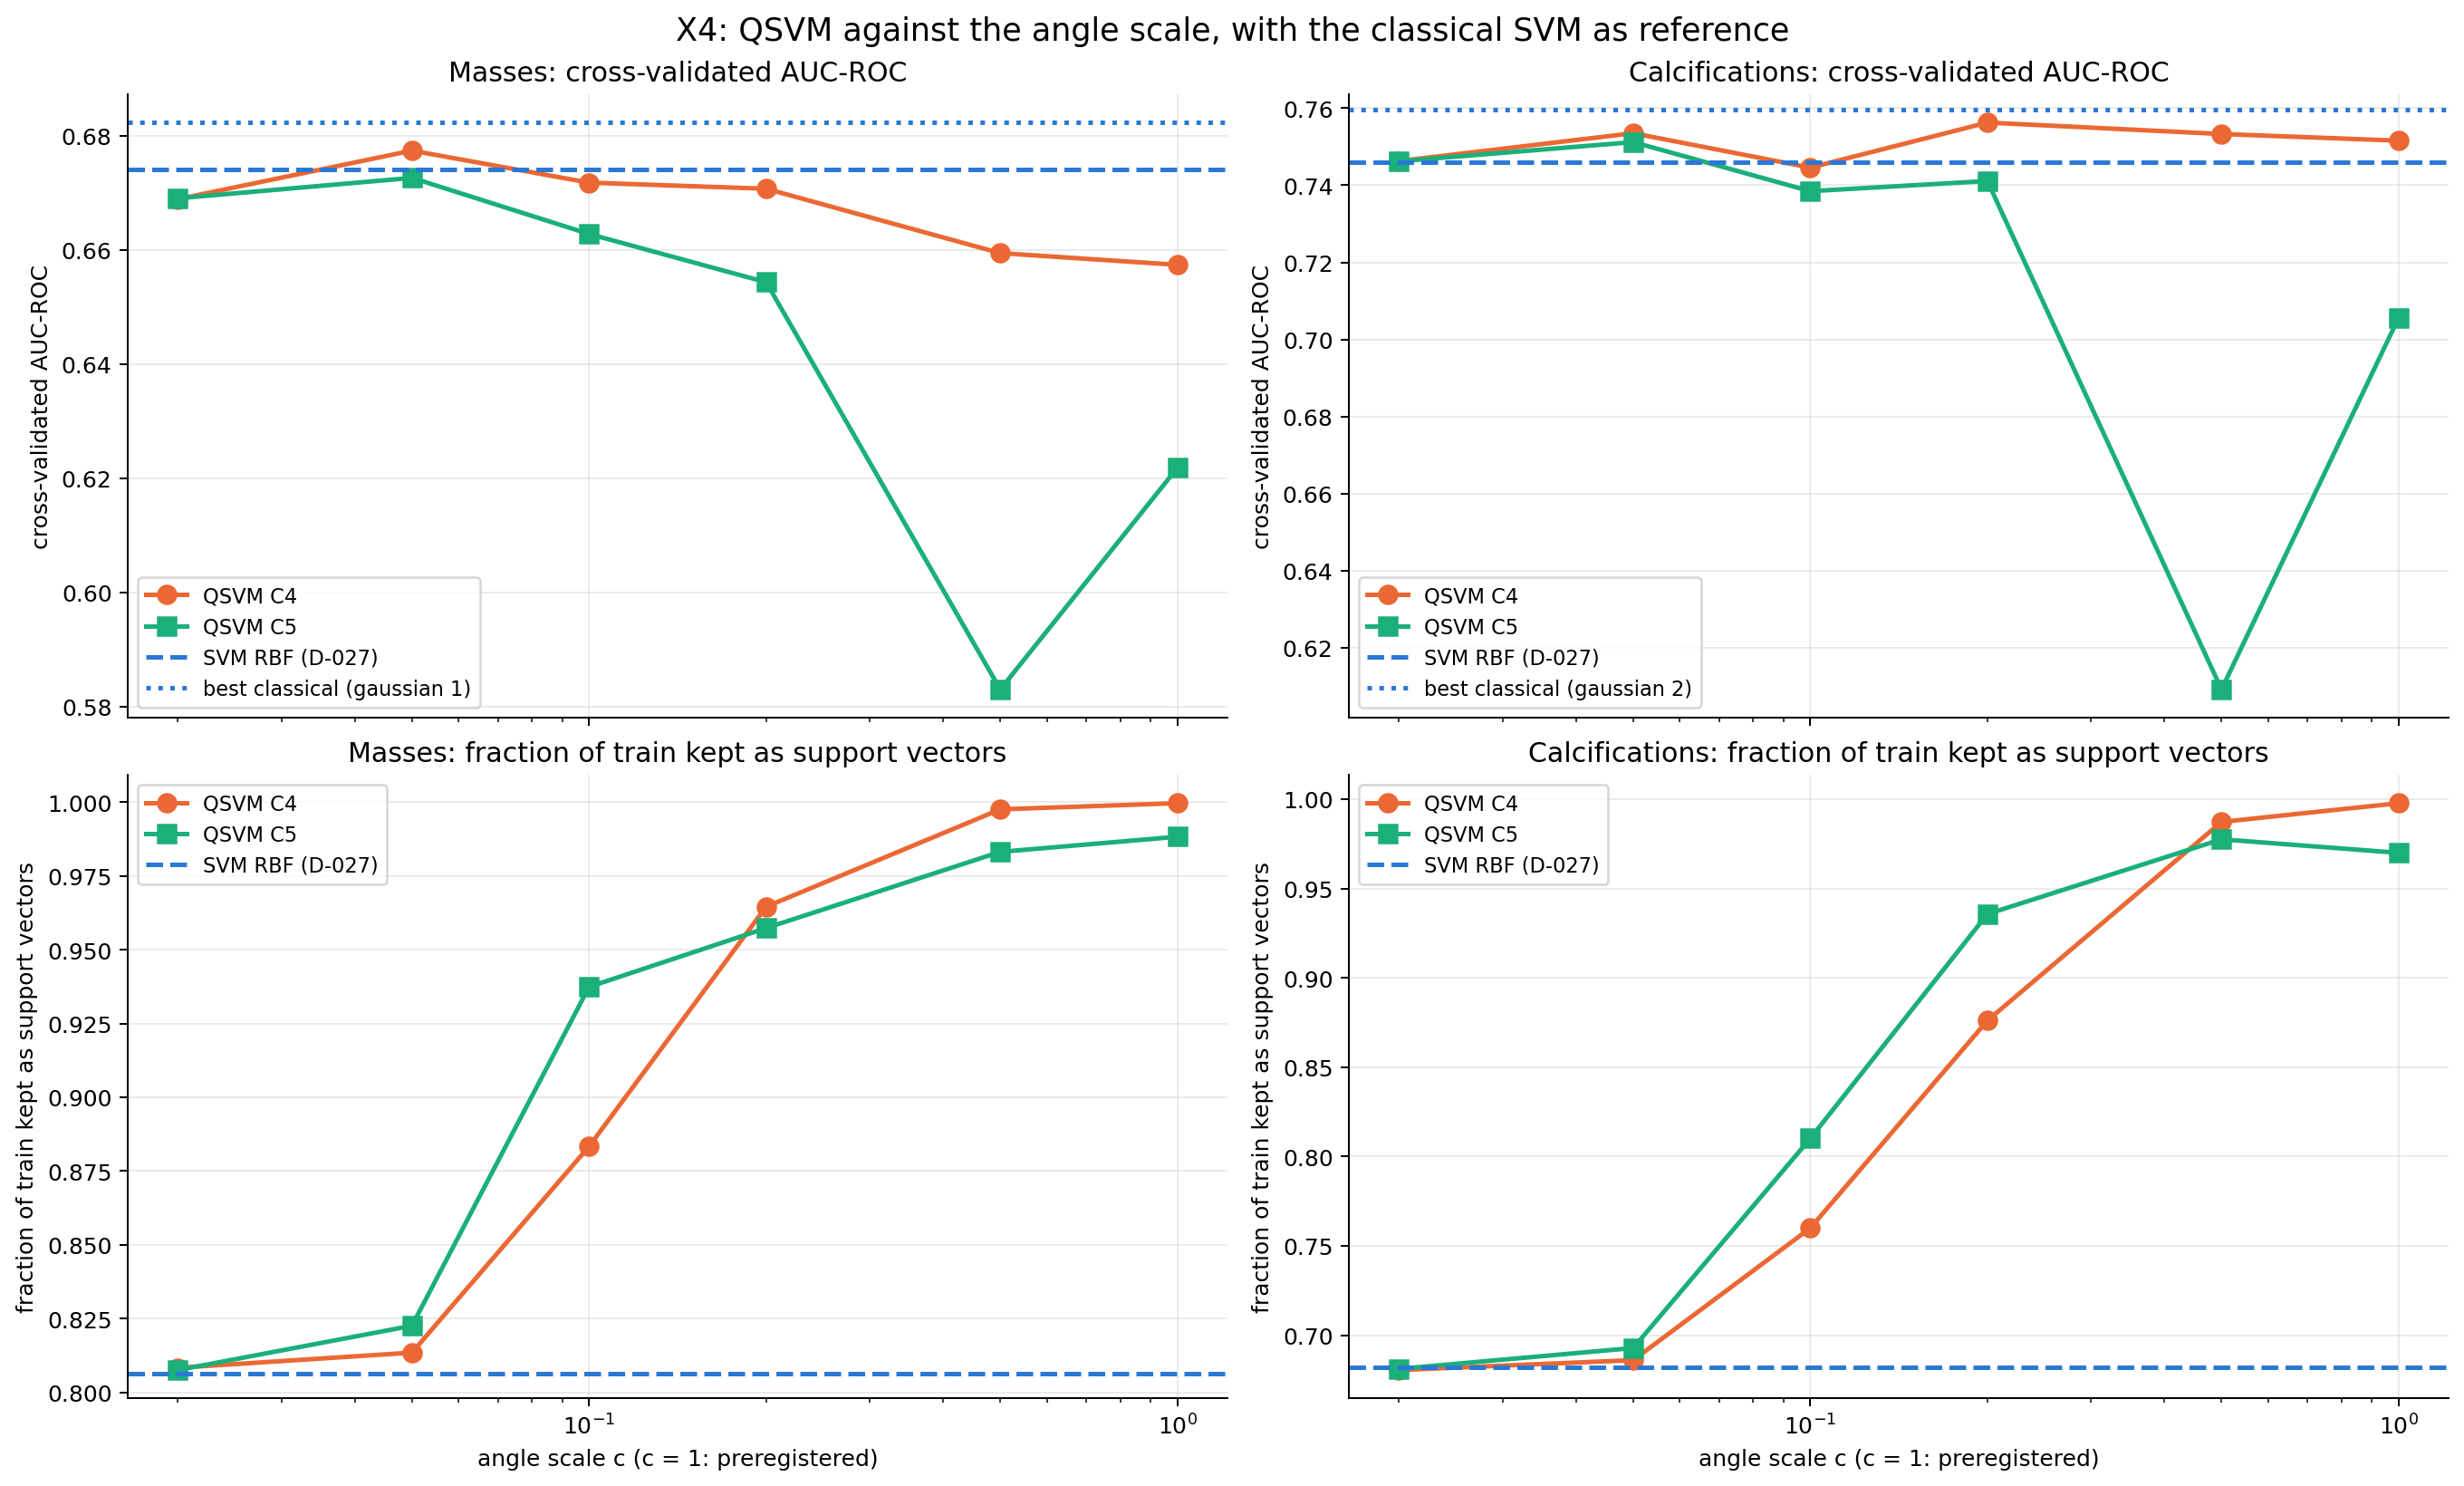
\includegraphics[width=\textwidth]{Figures/X4_qsvm_scale.png}
% fuente: H-044
\caption{Desempeño en clasificación del algoritmo QSVM frente a variaciones en el factor de escala angular $c$ (Experimento X4), contrastado con la referencia clásica de SVM con kernel gaussiano RBF.}
\label{fig:anx_x4_qsvm_scale}
\end{figure}

\begin{figure}[H]
\centering
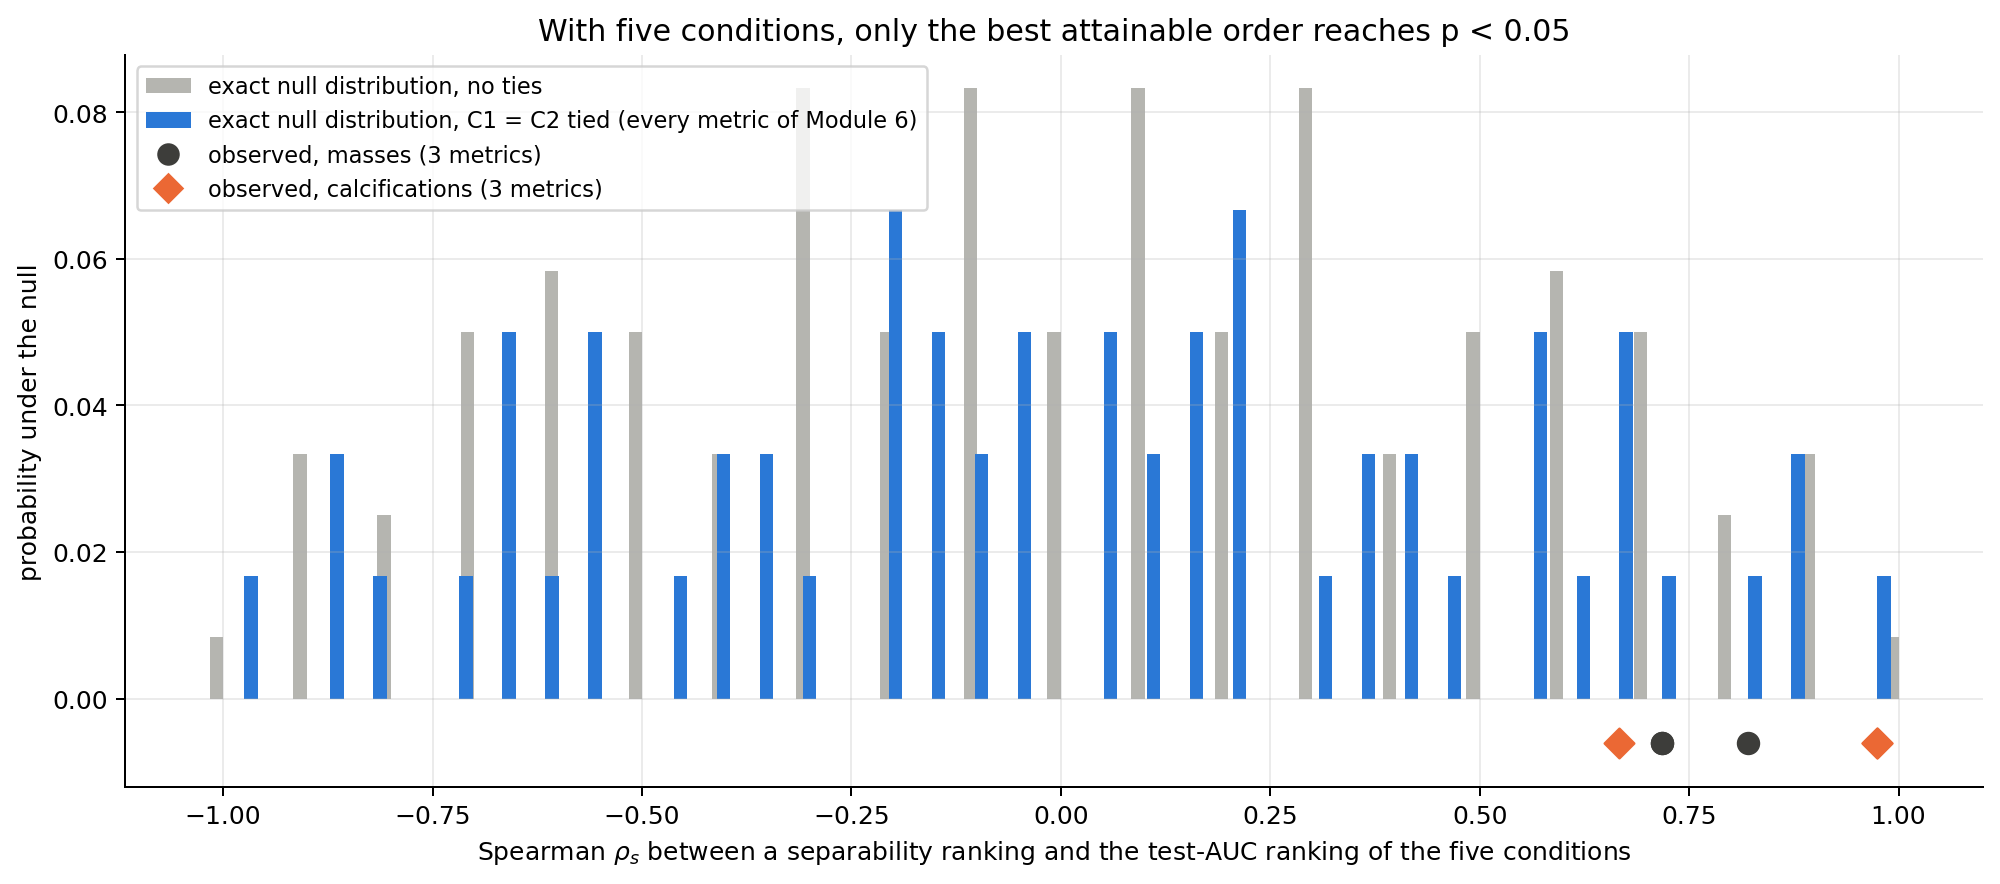
\includegraphics[width=0.85\textwidth]{Figures/M8_spearman_null.png}
% fuente: H-049
\caption{Distribución nula exacta del estadístico de correlación de Spearman $\rho_s$ generada a partir de las 120 permutaciones exhaustivas de las cinco condiciones experimentales con rangos promedio por empates (Módulo 8).}
\label{fig:anx_m8_spearman_null}
\end{figure}
